\documentclass[conference]{IEEEtran}
\IEEEoverridecommandlockouts

\usepackage{algorithmic}
\usepackage{amsmath, amssymb, amsfonts}
\usepackage{cite}
\usepackage{float}
\usepackage{graphicx}
\usepackage{hyperref}
\usepackage{textcomp}
\usepackage{xcolor}

\def\BibTeX{{\rm B\kern-.05em{\sc i\kern-.025em b}\kern-.08em
    T\kern-.1667em\lower.7ex\hbox{E}\kern-.125emX}}

\begin{document}

\title{Comparative Study of Medical Information Retrieval Approaches}

\graphicspath{ {./images/} }

\makeatletter
\newcommand{\linebreakand}{%
  \end{@IEEEauthorhalign}
  \hfill\mbox{}\par
  \mbox{}\hfill\begin{@IEEEauthorhalign}
}
\makeatother

\author{
    \IEEEauthorblockN{Davin Jason Evan Raharjo}
    \IEEEauthorblockA{\textit{Department of Computer Science} \\
    \textit{and Electronics} \\
    \textit{Universitas Gadjah Mada} \\
    Yogyakarta, Indonesia \\
    davinjasonevanraharjo@mail.ugm.ac.id}
    \and
    \IEEEauthorblockN{Asyraf Nur Ardliansyah}
    \IEEEauthorblockA{\textit{Department of Computer Science} \\
    \textit{and Electronics} \\
    \textit{Universitas Gadjah Mada} \\
    Yogyakarta, Indonesia \\
    asyrafnurardliansyah@mail.ugm.ac.id}
    \and
    \IEEEauthorblockN{Isneyri Arsyadani}
    \IEEEauthorblockA{\textit{Department of Computer Science} \\
    \textit{and Electronics} \\
    \textit{Universitas Gadjah Mada} \\
    Yogyakarta, Indonesia \\
    isneyriarsyadani@mail.ugm.ac.id}
}

\maketitle

\begin{abstract}
    soon
\end{abstract}

\begin{IEEEkeywords}
    soon
\end{IEEEkeywords}

\section{Introduction}

The increasing demand for accessible health information has made Medical Information Retrieval (IR) a crucial field in contemporary healthcare. As healthcare decisions increasingly rely on information availability, both healthcare professionals and the general public seek efficient systems to facilitate this access. Medical IR plays a pivotal role in supporting these needs by providing tailored information that can guide decision-making and health education. The evolution of medical IR has seen a shift towards user-centered approaches, emphasizing the importance of addressing the diverse requirements of different user groups, ranging from patients to specialized clinicians.

Recent advancements in medical IR research have focused on enhancing the relevance and accuracy of retrieved information through innovative methodologies. Among these, graph-based models have emerged as a powerful tool for representing complex medical knowledge, enabling systems to understand relationships between various medical concepts. Furthermore, techniques in terminology extraction are being utilized to improve the retrieval of domain-specific information. Clinical decision support systems, which integrate data and algorithms to assist healthcare professionals, also represent a significant stride towards optimizing medical IR. These developments underline the importance of creating personalized IR systems that take into account the unique contexts and needs of users.

Despite the promising advancements in medical IR, several challenges remain that must be addressed to ensure effective implementation. Diverse user needs pose a significant hurdle, as different users require varying levels of detail and types of information. Additionally, the varying medical knowledge of users necessitates that information is presented in an accessible manner, catering to both experts and laypeople. Language barriers further complicate this landscape, as much of the medical content is predominantly in English, limiting access for non-English speakers. Moreover, the complexity of health records, which often consist of varied formats such as clinical notes and pathology data, requires sophisticated retrieval methods. Finally, ensuring the reliability and accuracy of retrieved medical information is critical, as it directly impacts health decisions. Addressing these challenges is essential for the advancement of Medical IR and its ability to improve healthcare outcomes.

\section{Research Method}

This research uses a literature review approach based on previous research on Medical Information Retrieval (IR). The literature review method used in this study is Preferred Reporting Items for Systematic Reviews and Meta-Analyses (PRISMA) method. This method consists of several steps: identification, screening, eligibility, and inclusion. Figure \ref{fig:PRISMA} shows the steps of the PRISMA method.

\begin{figure}[ht!]
    \centering
    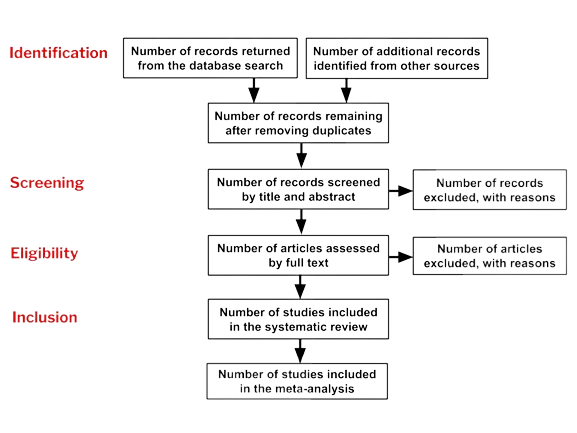
\includegraphics[scale=.4]{PRISMA.png}
    \caption{Steps of the PRISMA method}
    \label{fig:PRISMA}
\end{figure}

The PRISMA (Preferred Reporting Items for Systematic Reviews and Meta-Analyses) method is a standardized framework designed to enhance the transparency and reproducibility of systematic reviews. It is widely utilized to report the selection process of studies systematically and objectively, ensuring that researchers include relevant evidence while excluding unsuitable studies. The method comprises four primary stages: Identification, Screening, Eligibility, and Inclusion, which guide the researcher in narrowing the scope of the studies to be reviewed.

In the Identification stage, all potential studies are collected by searching databases and other sources. At this step, duplicate entries are removed to avoid redundancy. Papers are collected from several journal databases, such as ScienceDirect, Scopus, arXiv, Springer. In order to retrieve the appropriate research papers, we use advanced search feature and keywords based on our main topic. Our query consists of "Information Retrieval", "Medic", "Enhance", where three of them are connected using the AND operator. "Medic" is expanded using the OR operator that links it to "Health" and "Knowledge", which is We also expand "Enhance" term with the same method, adding "Improve" and "Boost" terms. To narrow the studies we found from the query, we set a number of constraints, including English language, their release that is after 2010, research article type, tagged as Computer Science and Engineering domains. The remaining records then proceed to the Screening stage, where their titles and abstracts are evaluated based on predefined inclusion criteria. Studies not meeting these criteria are excluded, with reasons documented for transparency.

In the next stage, Eligibility, full texts of the remaining studies are thoroughly assessed to confirm their relevance and quality. Articles failing to meet the review criteria are excluded, ensuring only high-quality and relevant studies are retained. Finally, in the Inclusion stage, the selected studies form the basis of the systematic review. If applicable, the meta-analysis is conducted using a subset of these studies, providing quantitative insights by synthesizing data from multiple studies. This structured approach ensures rigor and clarity in systematic reviews.

\bibliographystyle{ieeetr}
\bibliography{references}

\end{document}
